% !TeX root = ../main.tex

\setlength{\parindent}{0em}
\chapter{Experiments}
\section{Data Generation Strategy Comparison}
The first set of experiments focused on evaluating different strategies for generating training data, with the goal of identifying which approach most effectively facilitates downstream summarization. Direct reasoning (V1), in which the teacher model was required to infer key elements and triples before producing the summary, consistently produced incomplete and incoherent outputs. Although some degree of logical consistency was maintained, the generated summaries often lacked sufficient coverage of important content, limiting their utility as high-quality training data.

An alternative stage-by-stage strategy (V2) was designed to mitigate these issues by splitting the generation process into multiple steps. Contrary to expectation, however, this approach worsened coherence and frequently led to “out-of-focus” summaries in which the generated key elements diverged substantially from the final summaries. This indicates that decomposing the generation into smaller stages can actually amplify inconsistencies, making it difficult for the student model to learn meaningful reasoning patterns.

In contrast, the summary-first strategy (V3) demonstrated clear advantages. By first producing a coherent summary and then deriving supporting elements and triples, this method yielded the highest performance across all automatic and human-aligned evaluation metrics, including ROUGE, BERTScore, and Judge scores. These results suggest that ensuring coherence at the summary level provides a stable foundation for subsequent reasoning tasks, which in turn improves both training efficiency and output quality. Table~\ref{tab:strategy_comparison} presents the quantitative comparison of the three strategies.

\begin{center}
    \captionof{table}{Performance Comparison by Data Generation Strategy}
    \label{tab:strategy_comparison}
    \resizebox{\columnwidth}{!}{
    \begin{tabular}{lccccc}
        \toprule
        Model & R-1 & B-F1 & Judge & R-2 & R-L \\
        \midrule
        4stg\_v3 & \textbf{45.5} & \textbf{77.9} & \textbf{70.3} & \textbf{24.3} & \textbf{37.6} \\
        4stg\_v1 & 43.8 & 76.8 & 64.0 & 22.1 & 35.5 \\
        4stg\_v2 & 37.6 & 69.4 & 65.1 & 17.5 & 23.4 \\
        \bottomrule
    \end{tabular}}
\end{center}

\section{Training Strategy Comparison}
The second set of experiments explored alternative training strategies, with particular attention to learning rate schedules and parameter-freezing techniques. A key finding was that adopting a non-decaying learning rate significantly improved model performance. This suggests that, unlike larger-scale models where decay is often beneficial to avoid overfitting, smaller student models benefit from maintaining a steady learning signal throughout training.
Another observation concerns the role of different parameter groups. Freezing only the attention layers or only the MLP layers still resulted in relatively strong performance, indicating that both components of the network contribute meaningfully to summarization ability. For example, the ``only\_mlp'' variant retained a high BERTScore (78.6\%), suggesting that attention-driven representations alone can sustain semantic fidelity.

By contrast, the application of LoRA, though successful in other low-resource fine-tuning scenarios, failed to provide improvements in this summarization setting. In fact, performance stagnated or slightly regressed. This result not only underscores the task-specific nature of parameter-efficient methods but also highlights a potential conflict between LoRA’s parameter expansion and the principle of maintaining a lightweight student model. The results of these comparisons are reported in Table~\ref{tab:training_strategy_comparison}.

{
    \captionof{table}{Performance Comparison by Training Strategy}
    \label{tab:training_strategy_comparison}
    \centering
    \resizebox{\columnwidth}{!}{
    \begin{tabular}{lccccc}
        \toprule
        Model & R-1 & B-F1 & Judge & R-2 & R-L \\
        \midrule
        4stg\_v3-lr\_adj & \textbf{48.4} & \textbf{79.3} & 72.8 & \textbf{25.7} & \textbf{40.1} \\
        4stg\_v3-lr\_adj-only\_mlp & 46.6 & 78.6 & 71.5 & 24.2 & 38.4 \\
        4stg\_v3-lr\_adj\_lora & 45.6 & 78.0 & \textbf{73.6} & 23.3 & 37.4 \\
        4stg\_v3 & 45.5 & 77.9 & 70.3 & 24.3 & 37.6 \\
        4stg\_v3-lr\_adj-only\_attn & 45.2 & 77.8 & 69.1 & 23.0 & 37.1 \\
        \bottomrule
    \end{tabular}}
}

\section{Curriculum Stage Comparison}
The final set of experiments investigated the influence of curriculum learning, particularly the number of curriculum stages, on model performance. The findings reveal a nuanced picture. When trained without a decaying learning rate, models with a single stage occasionally achieved marginally higher ROUGE-1 scores compared to those trained with multiple stages. However, multi-stage setups (four or five stages) consistently yielded more accurate Traditional Chinese generation and greater stability in output quality. This suggests that while curriculum depth may not always maximize surface-level evaluation scores, it enhances the stylistic fidelity and robustness of the generated summaries.
Tables~\ref{tab:stage_lr_decay}--\ref{tab:stage_no_lr_decay} summarize these results, and Figure~\ref{fig:zh_tw_result} illustrates the proportion of Traditional Chinese in outputs among different models, especially in terms of improvements.

% \begin{table}[ht]
%     \centering
%     \caption{Performance of Different Stage Numbers with Decaying Learning Rate}
%     \begin{tabular}{lccccc}
%         \toprule
%         MODEL & R-1 & B-F1 & Judge & R-2 & R-L \\
%         \midrule
%         Qwen2.5-0.5B\_4stg\_v3 & 45.5 & \textbf{77.9} & \textbf{70.3} & \textbf{24.3} & 37.6 \\
%         Qwen2.5-0.5B\_1stg\_v3 & \textbf{45.9} & 77.9 & 68.8 & 23.7 & \textbf{37.7} \\
%         \bottomrule
%     \end{tabular}
%     \label{tab:stage_lr_decay}
% \end{table}

% \begin{table}[ht]
%     \centering
%     \caption{Performance of Different Stage Numbers without Decaying Learning Rate}
%     \begin{tabular}{lccccc}
%         \toprule
%         MODEL & R-1 & B-F1 & Judge & R-2 & R-L \\
%         \midrule
%         Qwen2.5-0.5B\_1stg\_v4-lr\_adj & \textbf{47.0} & \textbf{78.8} & \textbf{75.9} & \textbf{24.5} & \textbf{38.9} \\
%         Qwen2.5-0.5B\_4stg\_v4-lr\_adj & 46.8 & 78.6 & 75.2 & 24.2 & 38.6 \\
%         Qwen2.5-0.5B\_5stg\_v4-lr\_adj & 46.5 & 78.6 & 75.1 & 23.9 & 38.3 \\
%         \bottomrule
%     \end{tabular}
%     \label{tab:stage_no_lr_decay}
% \end{table}

% \begin{figure}[htbp]  % h=here, t=top, b=bottom, p=page of floats
%     \centering
%     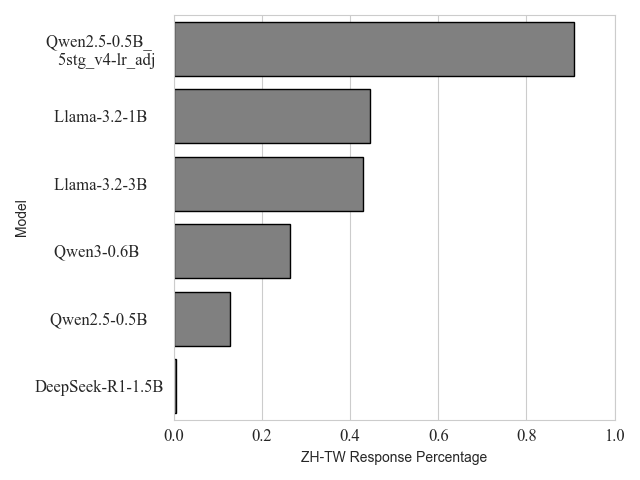
\includegraphics[width=0.7\textwidth]{figures/zh_tw_result_percentage_overall.png}
%     \caption{Proportion of Traditional Chinese responses generated by each model. The proposed 0.5B model with 5-stage curriculum achieves the highest ratio, surpassing even 3B models.}
%     \label{fig:zh_tw_result}
% \end{figure}

\vspace{0.75\baselineskip}
{
    \captionof{table}{Performance Comparison by Training Strategy}
    \label{tab:training_strategy_comparison}
    \centering
    \resizebox{\columnwidth}{!}{
    \begin{tabular}{lccccc}
        \toprule
        Model & R-1 & B-F1 & Judge & R-2 & R-L \\
        \midrule
        4stg\_v3-lr\_adj & \textbf{48.4} & \textbf{79.3} & 72.8 & \textbf{25.7} & \textbf{40.1} \\
        4stg\_v3-lr\_adj-only\_mlp & 46.6 & 78.6 & 71.5 & 24.2 & 38.4 \\
        4stg\_v3-lr\_adj\_lora & 45.6 & 78.0 & \textbf{73.6} & 23.3 & 37.4 \\
        4stg\_v3 & 45.5 & 77.9 & 70.3 & 24.3 & 37.6 \\
        4stg\_v3-lr\_adj-only\_attn & 45.2 & 77.8 & 69.1 & 23.0 & 37.1 \\
        \bottomrule
    \end{tabular}}
    \vspace{0.75\baselineskip}
}

% ------------------ TABLE 2.4 ------------------
{
    \captionof{table}{Performance of Different Stage Numbers with Decaying Learning Rate}
    \label{tab:stage_lr_decay}
    \centering
    \resizebox{\columnwidth}{!}{
    \begin{tabular}{lccccc}
        \toprule
        Model & R-1 & B-F1 & Judge & R-2 & R-L \\
        \midrule
        Qwen2.5-0.5B\_4stg\_v3 & 45.5 & \textbf{77.9} & \textbf{70.3} & \textbf{24.3} & 37.6 \\
        Qwen2.5-0.5B\_1stg\_v3 & \textbf{45.9} & 77.9 & 68.8 & 23.7 & \textbf{37.7} \\
        \bottomrule
    \end{tabular}}
}
\vspace{0.75\baselineskip}
\vspace{0.75\baselineskip}

% \begin{center}
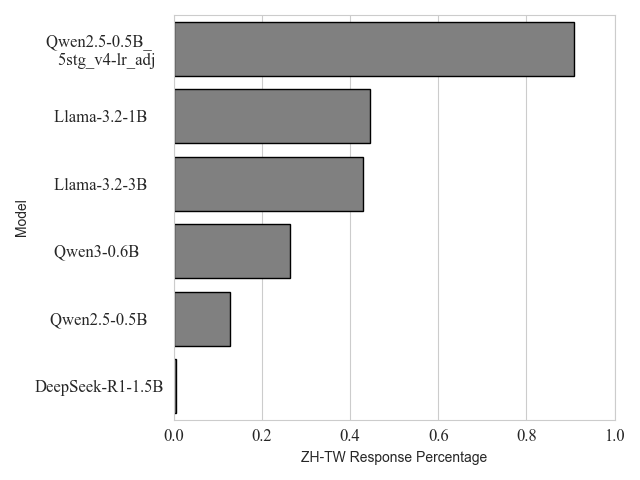
\includegraphics[width=\columnwidth]{figures/zh_tw_result_percentage_overall.png}
\captionof{figure}{Proportion of Traditional Chinese responses generated by each model. The proposed 0.5B model with 5-stage curriculum achieves the highest ratio, surpassing even 3B models.}
\label{fig:zh_tw_result}
% \end{center}

Furthermore, the benefits of curriculum learning appeared to depend heavily on the scale of pretraining. When large-scale pretraining was employed, curriculum learning only slightly improved summary quality. In contrast, with smaller pretraining datasets, curriculum learning provided substantial performance boosts, indicating that staged training helps compensate for weaker initial representations by guiding the model through progressively more complex tasks. As shown in Table~\ref{tab:custom_pretrain_stage_comparison}, the 4-stage curriculum model (Custom-pretrained-4stg\_v3-lr\_adj) consistently outperforms the single-stage counterpart across most metrics, particularly in ROUGE-1 and Judge scores, highlighting the effectiveness of gradual task progression in low-resource pretraining scenarios.

% \begin{table}[ht]
%     \centering
%     \caption{Performance of Custom Pretrained Models with Different Curriculum Stages}
%     \begin{tabular}{lccccc}
%         \toprule
%         Model & R-1 & B-F1 & Judge & R-2 & R-L \\
%         \midrule
%         Custom-pretrained-4stg\_v3-lr\_adj & \textbf{13.3} & \textbf{50.6} & \textbf{0.9} & \textbf{1.8} & 4.0 \\
%         Custom-pretrained-1stg\_v3-lr\_adj & 11.8 & 50.5 & 0.6 & 1.5 & \textbf{5.0} \\
%         \bottomrule
%     \end{tabular}
%     \label{tab:custom_pretrain_stage_comparison}
% \end{table}


% ------------------ TABLE 2.5 ------------------
{
    \captionof{table}{Performance of Different Stage Numbers without Decaying Learning Rate}
    \label{tab:stage_no_lr_decay}
    \centering
    \resizebox{\columnwidth}{!}{
    \begin{tabular}{lccccc}
        \toprule
        Model & R-1 & B-F1 & Judge & R-2 & R-L \\
        \midrule
        Qwen2.5-0.5B\_1stg\_v4-lr\_adj & \textbf{47.0} & \textbf{78.8} & \textbf{75.9} & \textbf{24.5} & \textbf{38.9} \\
        Qwen2.5-0.5B\_4stg\_v4-lr\_adj & 46.8 & 78.6 & 75.2 & 24.2 & 38.6 \\
        Qwen2.5-0.5B\_5stg\_v4-lr\_adj & 46.5 & 78.6 & 75.1 & 23.9 & 38.3 \\
        \bottomrule
    \end{tabular}}
}

